% Chapter Template

\chapter{Ensayos y resultados} % Main chapter title

\label{Chapter4} % Change X to a consecutive number; for referencing this chapter elsewhere, use \ref{ChapterX}

%----------------------------------------------------------------------------------------
En este capítulo se muestran los principales ensayos realizados y sus resultados, para verificar el cumplimiento de los requisitos. Además, se incluye un caso de uso completo.

%----------------------------------------------------------------------------------------
%	SECTION 1
%----------------------------------------------------------------------------------------

\section{Pruebas unitarias}
\label{sec:pruebasUnitarias}

\subsection{Calibración del electrodo}

Para la validación del proceso de calibración del electrodo se utilizó el banco de pruebas que muestra la figura \ref{fig:bancoPruebasCalibracion}, y se procedió a realizar el proceso de calibración.

\begin{figure}[htbp]
	\centering
	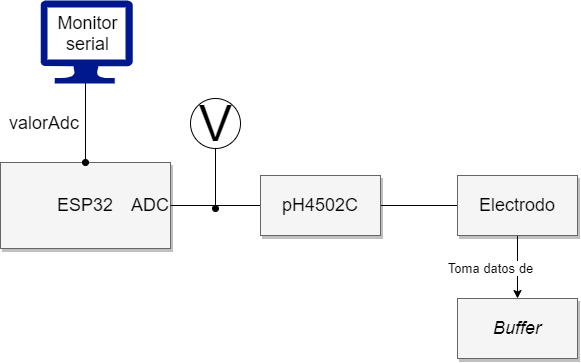
\includegraphics[width=0.7\textwidth]{./Figures/bancoPruebasCalibracion.png}
	\caption{Banco de pruebas para la calibración del electrodo.}
	\label{fig:bancoPruebasCalibracion}
\end{figure}

La tabla \ref{tab:ensayoCalibracion} muestra las mediciones correspondientes a la diferencia de potencial entregada por módulo pH4502C y al valor leído por el ADC para cada unos de los valores de los \textit{buffers}, en un ambiente con temperatura de 25 °C.

\begin{table}[h]
	\centering
	\caption[Resultados calibración]{Resultados obtenidos durante el proceso de calibración}
	\begin{tabular}{l c c }    
		\toprule
		\textbf{\textit{Buffer} [pH]} & \textbf{Salida pH4602C [V] }	&    \textbf{Lectura ADC}  \\
		\midrule
		4 	& 2,635 & 3050 \\		
		7	& 2,172 & 2455 \\
		10	& 1,877 & 2120 \\
		\bottomrule
		\hline
	\end{tabular}
	\label{tab:ensayoCalibracion}
\end{table}

A partir de los datos obtenidos, se puede graficar la recta de ajuste que relaciona el valor de pH con el valor de medido por el ADC, como se muestra en la figura \ref{fig:rectaADC}. Los valores de pendiente y ordenada al origen calculados en el ESP32 fueron visualizados por el monitor serial, y se obtuvo -0,0063 para el valor de la pendiente m, y 22,98 para el valor de la ordenada al origen b. 

\begin{figure}[htbp]
	\centering
	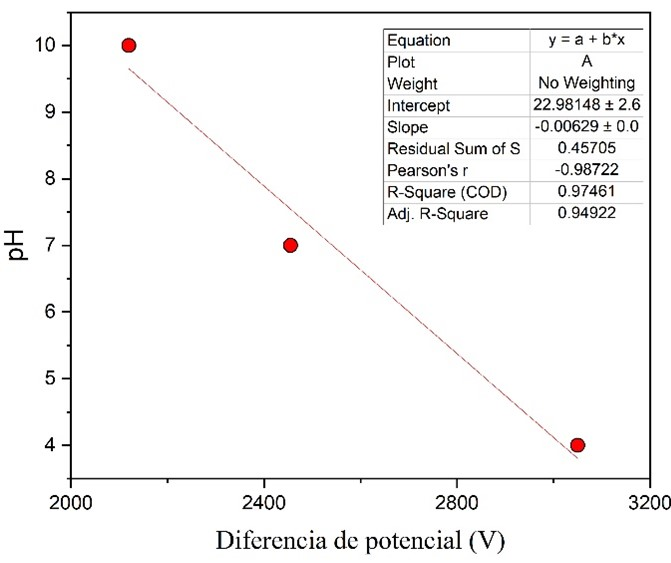
\includegraphics[width=0.7\textwidth]{./Figures/rectaADC.jpg}
	\caption{Relación entre el pH y el valor convertido por el ADC.}
	\label{fig:rectaADC}
\end{figure}

Luego de repetir el ensayo, se obtuvo que el error en la medición del potencial de salida del módulo pH4502C es de +/- 1 mV y luego de la conversión a pH el error es de +/- 0,1 pH a temperatura ambiente. 

\subsection{Calibración del volumen inyectado por la bomba}

En el diseño del prototipo, el control de bomba se realiza utilizando un esquema de lazo abierto, es decir que, cuando se inyecta líquido, el microcontrolador  no realiza una medición del caudal o del volumen que fue desplazado. A raíz de esto, surge la necesidad de establecer una relación entre la cantidad de pasos que realiza el motor y la cantidad de volumen que inyecta la bomba, para así poder tener una unidad de medida y verificar si cumple con los requerimientos establecidos. Esta relación es difícil de obtener de manera teórica mediante el uso de modelos, por lo que se decidió realizar una serie de dosificaciones de un líquido de densidad conocida, y pesar la cantidad dosificada para determinar el volumen. En banco de pruebas utilizado para realizar este ensayo se muestra en la figura \ref{fig:bancoPruebasBomba}. En este proceso el fluido a dosificar fue agua de red domiciliaria, con una densidad estimada de 1 g/mL y se utilizó una balanza de dos decimales con un error de ±0,01 g, recogiendo el fluido en un vaso de precipitado previamente tarado.

\begin{figure}[htbp]
	\centering
	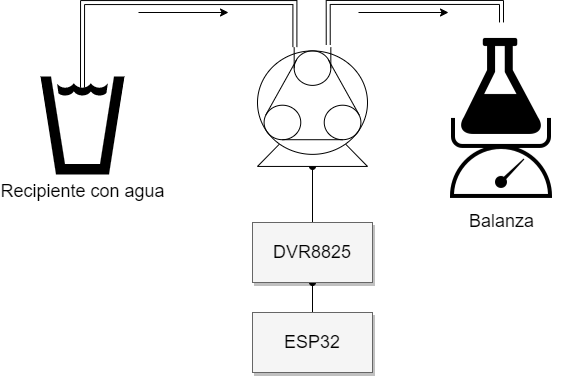
\includegraphics[width=0.7\textwidth]{./Figures/bancoPruebasBomba.png}
	\caption{Banco de pruebas para la calibración de la bomba.}
	\label{fig:bancoPruebasBomba}
\end{figure}

Se realizaron 10 dosificaciones, cada una de las cuales implicó una cantidad de 2500 pasos para el motor, a una velocidad constante de 93,75 rpm. Se registró el peso y se taró nuevamente la balanza para todas las dosificaciones. Esta relación entre el número de pasos y las mediciones de masa se muestra en la tabla \ref{tab:ensayoBomba}, y la serie de mediciones arroja un peso medio de 0,70 g con un desvío de ± 0,01 g.

\begin{table}[h]
	\centering
	\caption[Dosificaciones]{Dosificaciones para el cálculo de volumen por paso.}
	\begin{tabular}{l c }    
		\toprule
		\textbf{Número de dosificación} & \textbf{Peso [g] } \\
		\midrule
		1 	& 0,69 \\	
		2	& 0,70 \\
		3	& 0,69 \\
		4	& 0,69 \\
		5	& 0,71 \\
		6	& 0,70 \\
		7	& 0,69 \\
		8	& 0,69 \\
		9	& 0,70 \\
		10	& 0,69 \\
		\bottomrule
		\hline
	\end{tabular}
	\label{tab:ensayoBomba}
\end{table}

\section{Validación y verificación}
\label{sec:validacionVerificacion}

Para la validación del prototipo se desarrolló un caso de uso que incluyó los siguientes pasos:
\begin{itemize}
	\item Calibración del electrodo con los 3 \textit{buffers}.
	\item Configuración del volumen de corte.
	\item Proceso de limpieza.
	\item Titulación de 50 mL de HCI 0,0500 M con NaOH 0,100 M.
	\item Visualización de resultados en memoria micro SD y página web.
\end{itemize}




